\documentclass{article}

\usepackage{graphicx}
\usepackage{amsmath}
\usepackage{color}
\usepackage{algorithm}
\usepackage{hyperref}

\newcommand{\hl}[1]{\colorbox{yellow}{#1}}
\newcommand{\hlp}[1]{\hl{#1}}
\newcommand\tab[1][1cm]{\hspace*{#1}}
\graphicspath{{images/}}


\newif
\ifpicture

\picturetrue

\begin{document}
\pagenumbering{gobble}

\begin{titlepage}
	\title{2D Image Space-Time Blending Using Textures}
	\date{23rd January 2017}
	\author{Felix Marrington-Reeve}
	\maketitle
	\ifpicture
	\begin{figure}[h!]
	\center{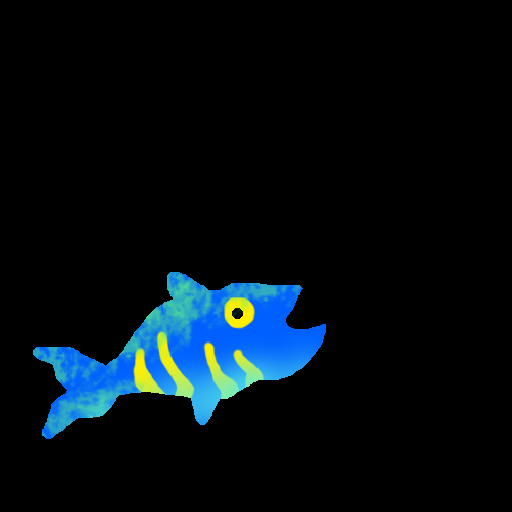
\includegraphics[width=0.3\linewidth]{fish_evolve_1.png}  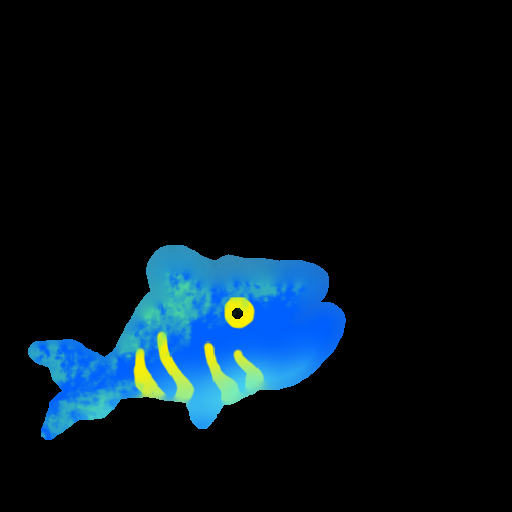
\includegraphics[width=0.3\linewidth]{fish_evolve_2.png}  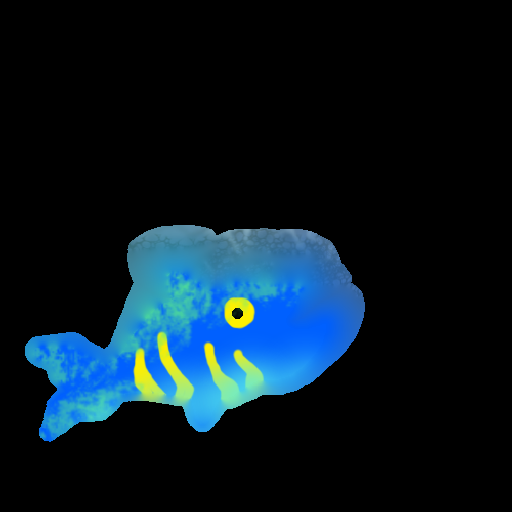
\includegraphics[width=0.3\linewidth]{fish_evolve_3.png}}
	\center{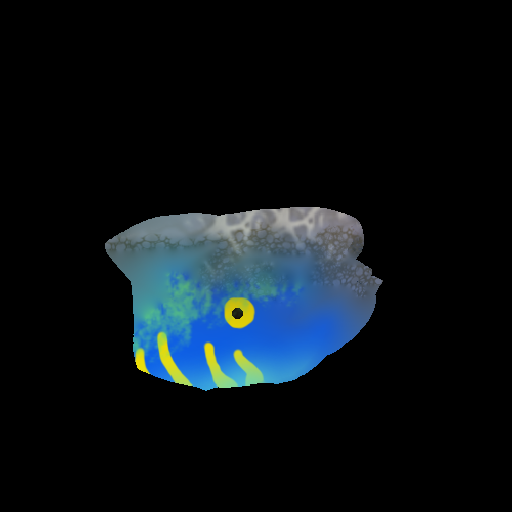
\includegraphics[width=0.3\linewidth]{fish_evolve_4.png}  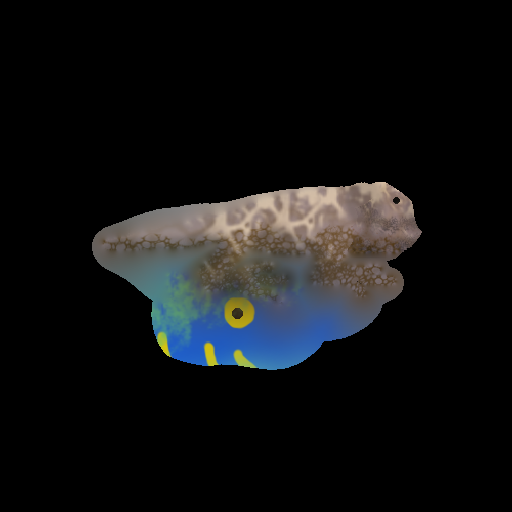
\includegraphics[width=0.3\linewidth]{fish_evolve_5.png}  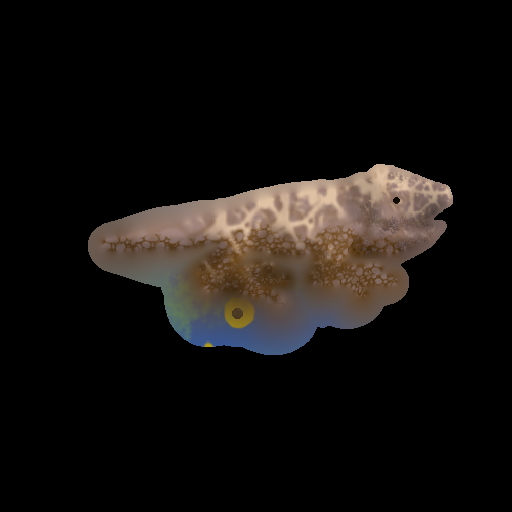
\includegraphics[width=0.3\linewidth]{fish_evolve_6.png}}
	\center{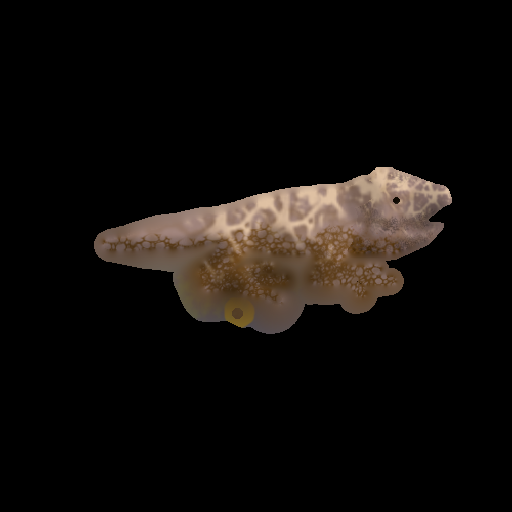
\includegraphics[width=0.3\linewidth]{fish_evolve_7.png}  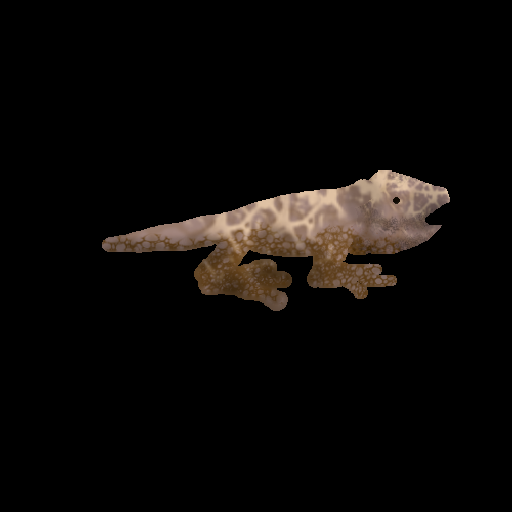
\includegraphics[width=0.3\linewidth]{fish_evolve_8.png}  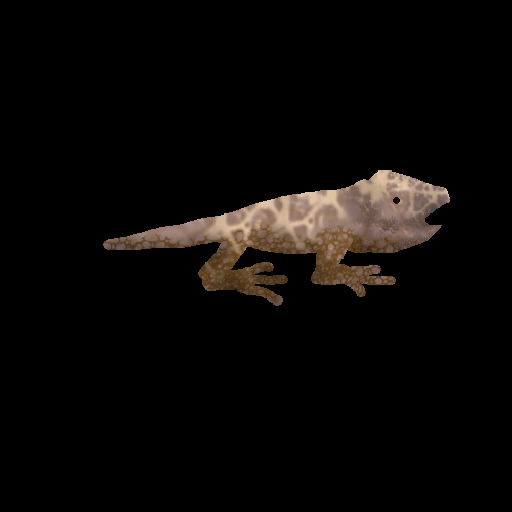
\includegraphics[width=0.3\linewidth]{fish_evolve_9.png}}
	%\caption{Blend from a user defined drawing, including shape and texture}
	\label{fig:fish}
	\end{figure}
	\fi
	\center{Supervisor: Valery Adzhiev}
	\newpage
	\tableofcontents
\end{titlepage}


\newpage
\pagenumbering{arabic}

\section{Abstract}
This is the abstract bla bla bla

\section{Introduction}
Heterogeneous object metamorphosis is a complex problem in animation. While there are a number of methods to creating a blend between two 2D shapes, many methods have disadvantages such as polygonal correspondence or requiring shapes to be defined by strokes rather than something more intuitive. Techniques that allow for blending without these restrictions tend not to allow for complex attributes such as textures. The aim of this paper is to research and develop a method for blending between two images to create a series of inbetween images which allows for attribute blending; in this case two textures, one applied to each keyframe, which can be blended between.

In \cite{space-time blending}, Pasko et al. put forward a method for blending between shapes that can be applied to both 3D and 2D spaces, and requires no correspondence in topology or position for the metamorphosis to work. In cases where such assumptions are not required, attributes such as colour are still difficult to blend between, particularly in areas of the output where the initial shapes do not overlap. A similar problem is found in automatic 2D inbetweening, where it is often not enough for images to be defined by 2D pixels which are often used to represent a 3D space \hl{[REFERENCE TO MATHSY PETER]}.

Even once the metamorphosis of shape is calculated, there is very little research on bending between other attributes of the objects, such as colour. If the 2 input images or keyframes have textures on them, there are currently no methods for blending between arbitrary raster images. This report presents a method for blending between 2 images with textures applied to them.

\section{Background and Alternative Approaches to Metamorphosis}
\subsection{Image Prediction}
Motion estimation can be relatively easily achieved using polynomial expansion \hl{[http://www.diva-portal.org/smash/get/diva2:273847/FULLTEXT01.pdf]}. The OpenCV library provides some open source functions that allow motion flow to be calculated and used for naive image prediction, such as the next frame or in between frames \textit{Fig \ref{fig:webcam}}.\\

\ifpicture
\begin{figure}[h!]
\center{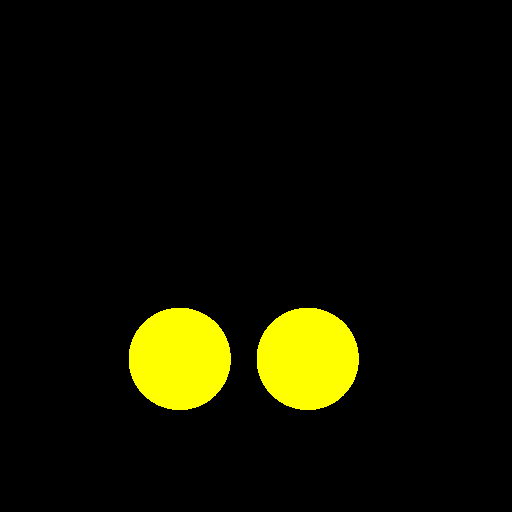
\includegraphics[width=0.4\linewidth]{rgb_1.png}}
\caption{IMAGE CAPTION}
\label{fig:webcam}
\end{figure}
\fi

\hl{WEBCAM IMAGES}\\\\
\textbf{Step 1:\\
\tab Use OpenCV to calculate a dense optical flow field.\\
Step 2:\\
\tab Use the flow result to predict the next frame:\\
\tab \tab Copy the 2nd frame used in prediction\\
\tab \tab For each pixel:\\
\tab \tab \tab Read “flow” vector of the pixel\\
\tab \tab \tab Copy the pixel to a position offset by the flow x and y values\\
\tab \tab Return the newly created frame}

This approach works fairly well on simple images with basic motion and can be used to get inbetween frames or predict the next frame.\\

\hl{Square motion images}

Frame prediction and inbetweening was very effective in the case of \hl{figure SOMETHING}, in which the colours, shapes and movement are very simple. Although the algorithm is basic, in specialised cases this may be suitable for interpolating or predicting frames. As far as I know this is the only program of this form, and as such provides an innovative alternative to rendering new frames if the animation is very limited.

However, due to its simplistic nature, it creates artefacts on more complex images and motions, since as parts move “out of the way”, they reveal areas where new information needs to be filled in and as such is not appropriate for the aim of this project, such as in \hl{FIGURE SOMETHING}.

\hl{Insect Motion Images}

\subsection{Texture Synthesis / Wave Function Collapse}
One Possible solution to the issue of missing information is to use the images to create possible or probable replacements for areas of the image with no information. 

\hl{Paul Merrel http://graphics.stanford.edu/~pmerrell/thesis.pdf}

\hl{Paul Harrison http://logarithmic.net/pfh-files/thesis/dissertation.pdf}

Some of these ideas are implemented in the program, “WaveFunctionCollapse” \hl{https://github.com/mxgmn/WaveFunctionCollapse}, which uses ideas from quantum physics to create an algorithm that can generate “locally similar” images to input images. By using a similar algorithm with a 3D array of pixels from a video, where the third dimension is time, it might be possible to get “locally similar” output frames as predictions or automatic inbetween images. Using this large 3d array, the program might be able to make more advanced predictions based on more than just the previous 2 frames.\\

\textbf{Step 1: Read an image sequence and create a 3D array of pixel colour and flow\\
Step 2: Read array values and create data structure suitable for wave function collapse\\
Step 3: Synthesise the next frame in the sequence based on likely flow and colours in the desired frame}

This approach, while theoretically interesting, will likely not produce any accurate results, as the wave function collapse algorithm is specifically used for “locally similar results”, rather than results that make logical sense in a wider context such as the whole frame or sequence. However, it is a new method that has not been explored before and might make for interesting future research.

\subsection{Alternative Approaches}
An early example of inbetweening 2D images can be found in Interactive Skeleton
Techniques for Enhancing Motion Dynamics in Key Frame Animation \hl{https://pdfs.semanticscholar.org/4849/b69b13b940604dbaa3ebc95ac953c3404463.pdf} where the authors present a system for morphing lines into different shapes and creating inbetweens. However, the line strokes must have correspondence and a skeleton must be set up in order to fully utilise the system.

A more modern solution can be found in Correspondence Specification Learned From Master Frames for Automatic Inbetweening (Jin and Geng) \hl{[link to Jin and Gen]} present an approach for automatic in betweens that relies on creating a 3D model from a front-view and side-view of a character, and on having accurate drawings of the 2D character in order to create correspondence between strokes. The strokes can be incorrectly annotated and there is no option for transitioning between radically different images such as drawings with radically different strokes or shapes.

\subsection{FRep Solids and Heterogeneous Objects}
An implicit shape can be represented by either $F(x, y)$ for 2D shapes or $F(x, y, z)$ for 3D shapes, where on the defining curve or surface $F(x, y) = 0$ in 2D or $F(x, y, z) = 0$ in 3D. An FRep solid is defined by primitives and operations, where $F \leq 0$. In [Space-time blending] Pasko et al. put forward a method which converts two $k$ dimensional input shapes into $(k+1)$ dimensional shapes in order to blend between them in the higher dimension. This allows inbetween models that do not rely on matching topology of the two inputs, due to their functional representation. In 2D:

\textbf{Two shapes are given using the x,y plane\\
Each shape is used as a cross section of a half cylinder in 3D space, by extending them in the z dimension, with space inbetween for the blend\\
The blending union operation is applied, this can be user controlled with different parameters\\
Using the z dimension as time, take cross sections of the shape along the z axis to display a smooth blend between the 1st and second shape}

The implementation in 3D is essentially the same, but raises the shapes into 4D and uses the 4th axis as time.

By blending using functional representation and this metamorphosis method, it is possible to create in between frames that have the following advantages over the other methods mentioned.
\begin{itemize}
\item The keyframes need not overlap or have similar shapes or colours
\item Textures should be implemented and a method or method of blending between textures should be present, including areas where no texture information is present, such as outside of both keyframes’ shapes
\item A relatively high level of user control should be possible
\end{itemize}

Heterogeneous objects which include both the shape and attributes of the object, such as colour, can also be represented using signed-distance fields. Object-Space Multiphase Implicit Functions \hl{http://i.cs.hku.hk/~yzyu/publication/OSMIF-sig2012.pdf} states that implicit functions have uses in entertainment, engineering and the medical industry. The potential that multiphase implicit functions have is also communicated, with implicit modeling that can represent different internal materials of objects. This allows the internal structure of objects to be modeled using implicit functions, which has further uses. This adds complexity to the space-time blending operations which is addressed in \hl{Space-Time Transfinite Interpolation (Bmth lectureres)} in which the authors propose interpolation of section attributes such as colour, as well as using blends with established correspondence between partitions and blends with no established correspondence. The authors also suggest a method for a summation of a voxel field, or a pixel array in 2D, for a weighted average of colours at the inbetween stage of the blend where colour is not explicitly defined.

The work of \hl{PASKOV ETC} is implemented in the following section, followed by an implementation of the paper's theoretical method for blending between textures. 

\section{Development}
I began to implement a similar set of 2D functions to the FRep program HyperFun \hl{[LINK]} in my own program, using C++. This began with a simple program in which functions can be written in GLSL to create a boolean image of the signed distance field that it creates. This allows an input of time to blend between two functions using the methods put forward in \hl{Real-Time Space-Time Blending with Improved User Control}, with a series of black and white output images.

\subsection{Single Colours}
Colours can be blended between using a simple \hl{transfinite interpolation ??} between the two initial states, where pixels’ colours are weighted by the absolute value of $f_{1}$ and $f_{2}$:

\begin{equation*}
c(t) = w_{1}(t) \cdot c_{1} + w_{2}(t) \cdot c_{2}
\end{equation*}
Where\\\\

$w_{1}(0) = 1$ and $w_{2}(0) = 0$ for $f_{1} \leq 0$ (on or inside G1)\\\\
$w_{1}(1) = 0$ and $w_{2}(1) = 1$ for $f_{2} \leq 0$ (on or inside G2)\\\\
$w_{1} + w_{2} = 1$\\

The interpolation uses initial constant colours, and as shown in \hl{[FIGURE]}, the colour change is non-linear and dependent on the shape of the two input shapes. The colour of the object can also be represented as a function of space, or $c_{1}(x, y)$ and $c_{2}(x, y)$ to two procedural textures that can be blended between.

The interpolation method should be dependent on the attribute being interpolated. In \hl{FIGURE} an example is shown of interpolating using the HSV colour space, rather than RGB. The colours are less intuitive as they are calculated by blending in the HSV space, causing unusual hues to appear as the colour is interpolated. In most cases the RGB colour space is more appropriate, although the option to use HSV to interpolate the colours can produce visually interesting results if desired

\hl{images of RGB/HSV}

\subsection{Partitions and Texturing}
Basic partitioning is possible using functional definitions for the colour of each object, using intersections of the original shape with sectional functions. There is no correspondence between partitions, and so the colour is calculated as follows, for the overall contribution of the object to the attribute at the given point:
\begin{equation*}
	c_{i}(x) = \sum_{j=1}^{N}\tilde{w_{j}}(x)\tilde{c_{j}} \over \sum_{j=1}^{N}\tilde{w_{j}}(x)
\end{equation*}
where $N$ is a number of partitions and the weight of each partition is give by $\tilde{w_{j}}(x) = {1 \over f_{j}(x)}$. Once this algorithm is implemented, it is relatively straightforward to implement a system where pixels or voxels of a provided texture can be used as numerous individual partitions, each with a given colour.

\hl{IMAGES}

The colours of the input textures ought to be defined only inside the input shapes. The colour of an output pixel is calculated using the distance to other pixels on the image, which allows a smooth blend between the two input textures.

Although a similar method is suggested in \hl{Space-Time Transfinite Interpolation of Volumetric Material Properties} I believe this to be the first implementation of this method, and it works well in practice, as shown in \hl{Figure Something}.

\hl{BALLS IMAGE}

\subsection{Alternative Colour Calculation Method}
An alternative implementation of generating colour is to use the colour of the closest point where $f \leq 0$ for each object and blend the result. This looks odd looking at the inside of the object but might seem more intuitive for certain applications such as looking at the surface of a 3D object for example, and retains the detail of the original surface while the shape expands. This is a relatively simple approach but is of my own design and I believe could be seen as useful in some situations where the internal structure of the blend is less important than the surface colour.

\hl{EQUATION?}
\hl{IMAGE EXAMPLE}

Another option in the program is to use a lower resolution version than the texture in order to preview the blend. This allows for faster results from the colour calculation, although it is significantly less accurate with lower resolutions \hl{[figURE SOMETHING]}

\hl{images}

\section{Image to SDF Conversion}
One area that \hl{Paskov et al} do not seem to have explored is the creation of Signed-Distance Fields from methods other than functions. As such, it is difficult to argue for the use of space-time blending, since it requires that shapes be defined by functional representations, which are often unintuitive without specialist software to create them. The 8SSEDT algorithm from \hl{A Note on Fast Raster Scan Distance Propagation on the Discrete Rectangular Lattice} is implemented, which takes a boolean raster grid and uses it to create a SDF.

This allows the user to draw an image with a black background for \textit{outside} the object and use textures of their choosing for \textit{inside} the object. This method is implemented to allow a more artist-friendly appraoch to creating the two keyframes of the blend. This algorithm is easy to incorporate into an FRep model as instead of using functions to create the implicit shape, a $SDF(x, y)$ function can be implemented which can be used to look up values once the SDF is generated. The result of this is the ability to generate non-trivial blends more easily, and it the implementation is entirely new for space-time blending.

\subsection{8SSEDT Algorithm}
The 8SSEDT algorithm is created by \hl{[REFERENCE]} and improved by Richard Mitton \hl{http://www.codersnotes.com/notes/signed-distance-fields/}

\hl{ALGORITHM}

\subsection{Further development}
In order to further improve the system it would be beneficial to integrate the functional representation that is shown in the tests in the paper. It would also be beneficial to focus on other areas that were not touched upon in the project, such as optimisation of the colour averaging algorithm, such as using voxels 

\section{Conclusion}

A method has been presented and implemented for allowing a blend between two raster images, that is not dependent on correspondence of attributes between them. It is the first implementation of the effect, and the first combination of converting images to signed-distance fields and then blending between them. The ability to use the closest point on the surface of the original shape is a new approach that, while simple, may have uses in 3 dimensions in particular in order to create a more intuitive surface of a model while it is going through space-time blending. The program is implemented in a user-friendly way that does not require functional representation of the shapes involved to create a blend, which I also believe to be the first implementation of the space-time blend using raster images.

\begin{thebibliography}{2}

%%%%%%%%%%%%%%%%%%%%%%%%%%%%%%%%%%
\bibitem{space-time blending}
Pasko, G., Pasko, A., and Kunii, T., 2004. Space-time Blending. \emph{Computer Animation and Virtual Worlds} [online]. Available from: \url{http://onlinelibrary.wiley.com/doi/10.1002/cav.12/abstract}
%first paper introducing the idea of space-time blending of frep solids
%lots of detailed explanation of process and implementation

\end{thebibliography}

\section{Appendix}
\subsection{2D Shapes, Operations and Transformations}

\end{document}